%%%%%%%%%%%%%%%%%%%%%%%%%%%%%%%%%%%%%%%%%%%%%%%%%%%%%%%%%%%%%%%%%%%%%%
% How to use writeLaTeX: 
%
% You edit the source code here on the left, and the preview on the
% right shows you the result within a few seconds.
%
% Bookmark this page and share the URL with your co-authors. They can
% edit at the same time!
%
% You can upload figures, bibliographies, custom classes and
% styles using the files menu.
%
%%%%%%%%%%%%%%%%%%%%%%%%%%%%%%%%%%%%%%%%%%%%%%%%%%%%%%%%%%%%%%%%%%%%%%

\documentclass[12pt]{article}

\usepackage{sbc-template}

\usepackage[round]{natbib}

\usepackage{indentfirst}
\usepackage{epigraph}

\usepackage{graphicx,url}

\usepackage[brazil]{babel}   
\usepackage[utf8]{inputenc}

\usepackage[table]{xcolor}
\usepackage{multirow}
\usepackage{scalefnt}
\usepackage{enumerate}
\usepackage{hyperref}     
\usepackage{array}
     
\sloppy

\title{API \emph{Web} de Geovisualização para Tratamento e Análise de Dados Espaciais}

\author{Yuri H. Martins\inst{1}, Ivre Marjorie R. Machado\inst{1}}
\address{PUC Minas em Contagem\\Bacharelado em Sistemas de Informação
\email{yurihm@hotmail.com, ivre.marjorie@gmail.com}
}

\begin{document} 

\maketitle

\begin{resumo} 

A necessidade de análise visual de dados de forma simplificada é uma realidade, devido à vasta quantidade de dados gerados diariamente, principalmente após o avanço da Internet e seus recursos tecnológicos. A geovisualização é uma poderosa ferramenta que auxilia na tomada de decisão para resolução de diversos tipos de problemas de grandeza espacial. Devido à existência de softwares complexos e limitados para esta análise, este trabalho tem por motivação auxiliar neste processo, permitindo que qualquer pessoa seja capaz de manipular dados e obter informações específicas. Para tanto, será desenvolvida uma API Web, com uma série de recursos construídos em JavaScript.

\end{resumo}

\begin{abstract}

The need for visual analysis of data in a simplified form is a reality, due to the vast amount of data generated daily, especially after the advancement of the Internet and its technological resources. Geovisualization’s a powerful tool that assists in decision making for solving various types of problems of spatial magnitude. Due to the existence of complex and limit softwares for this analysis, this job have a motivation to assist in this process, allowing anyone to be able to manipulate data and get specific information. Therefore, a Web API will be developed, with a series of resources built in JavaScript.

\end{abstract}
     
\section{Introdução}

O avanço da internet propiciou que sejam gerados cada vez mais dados referentes a diferentes áreas e setores de negócio no mundo. Termos como \emph{Big Data}\footnote{refere-se a um grande conjunto de dados armazenados.} e \emph{Internet of Things}\footnote{Internet das Coisas. Ideia de conectar à Internet os dispositivos eletrônicos utilizados no dia-a-dia.} são usados para justificar essa quantificação de informação. Uma vez que mais dados são gerados, mais difícil se torna fazer a interpretação e análise dos mesmos.

Conceitualmente, a visualização de dados é um conjunto de técnicas que permite a todas as pessoas que precisam de informações úteis para determinado fim, obter o valor imediato a partir de dados, seja eles qual for. A visualização de dados surgiu com o intuito de simplificar grandes quantidades de dados, reduzindo milhares de linhas a imagens e gráficos que possibilitem a compreensão das informações. O ser humano por si só não é capaz de processar várias informações ao mesmo tempo, sendo assim, ferramentas que auxiliem na análise visual de dados são cada vez mais necessárias, além de ser uma área de pesquisa que está em constante desenvolvimento.

Uma linha de discussão sobre esse tema são os dados de origem espacial. Esses dados se enquadram dentro do que é chamado de Geoprocessamento, sendo basicamente o uso de técnicas matemáticas e computacionais para tratar a informação. O processamento desses dados é realizado por meio de Sistemas de Informações Geográficas (SIGs). \citet{bdgeo} afirma que o uso do SIGs implica em escolher as representações computacionais mais adequadas para capturar a semântica de seu domínio de aplicação. Ainda diz que desenvolver um SIG significa oferecer um conjunto mais amplo possível de estruturas de dados e algoritmos capazes de representar a grande diversidade de concepções do espaço.

Novas tecnologias vinculadas a \emph{Web} foram surgindo, possibilitando que os SIGs pudessem receber novos tipos de dados, de diferentes formatos e meios, o tornando cada vez mais sofisticado e, consequentemente, mais complexo. Cada um possui suas bibliotecas de funções e procedimentos para tratar os dados que chegam, tornando o uso deste viável apenas a pessoas com experiência e de áreas relacionadas à computação e geografia. Usuários com menos conhecimento nestas áreas, por exemplo, não seriam capazes de utilizá-los facilmente. Além disso, a maioria desses sistemas são estáticos, não permitindo interação do usuário com o mesmo.

Atualmente existem algumas bibliotecas em JavaScript, como o caso do D3.js, que disponibilizam diversos recursos para visualização de dados, inclusive em formatos de mapas. Um tipo de mapa que é encontrado nessa biblioteca e é comumente usado na Cartografia são os mapas coropléticos\footnote{representação de uma superfície estatística por meio de áreas simbolizadas com cores, sombreamentos ou padrões de acordo com uma escala que representa a proporcionalidade da variável estatística em causa.}. Esse tipo de mapa é ideal para análises de dados que são delimitados por áreas (municípios, estados, regiões, etc.).

Ao tratar de assuntos relacionados a mapas, uma das primeiras aplicações que vem à cabeça é o Google Maps, que é um serviço gratuito para visualização de mapas e imagens de satélite da Terra \citep{googlemaps}. Ele dispõe de mecanismos que permitem que usuários leigos manipulem e interajam com os mapas, criando rotas, dando zoom, navegando entre locais, etc., sem necessidade de conhecimento específico. Esse tipo de usuário foi denominado de “neogeógrafos” por \citet{turner}, dizendo que essas pessoas não são especialistas, mas são capazes de produzir mapas. A facilidade que o avanço tecnológico proporcionou vem fazendo pessoas de diversas áreas de atuação migrarem de setores. \citet{armstrong} já havia afirmado isso ao defender que os geógrafos deveriam ser capazes de lidar com as tecnologias, pois se não assumissem as lideranças das pesquisas geográficas, profissionais de outras áreas o fariam.

Dadas funcionalidades como as existentes no D3.js e Google Maps, vê-se a viabilidade de criação de uma tecnologia que possua funcionalidades tais como estas e disponibilize recursos semelhantes aos que um SIG pode oferecer, dando ao usuário poder de trabalhar com informações em um mapa ou gráficos, de acordo com sua necessidade. Profissionais como geógrafos, professores e economistas utilizam dados espaciais como fonte de pesquisa. Uma plataforma com estas características seria de grande valia no auxílio à tomada de decisões, estudos e desencadeamento de pesquisas.

O grande objetivo deste projeto é a integração de um conjunto de recursos \emph{Web}, principalmente JavaScript, para construção de uma API de geovisualização interativa capaz de gerar a visualização de informações relacionadas ao meio geográfico (por exemplo, dados demográficos, PIB\footnote{Produto Interno Bruto.}, IDH\footnote{Índice de Desenvolvimento Humano.}, características populacionais, etc.). Esta API deverá acessar uma base de dados com mapas do território brasileiro e ser capaz de receber arquivos com dados referentes à região que o usuário escolher. Assim feito, haverá a leitura desses dados e confecção das informações em um mapa coroplético principal, com opções de configuração, como cores, intervalo de agrupamento dos dados e visualização temporal. Em segundo plano, haverá gráficos estatísticos dinâmicos que serão carregados com dados de acordo com as ações do usuário (cliques) no mapa principal.

Este trabalho está organizado em quatro seções. Na seção 2 é feita uma revisão literária, abrangendo os principais aspectos teóricos e conceituais relacionados ao tema proposto, focando em correlacionar o uso da tecnologia e a geografia analítica. A seção 3 apresenta os trabalhos relacionados ao tema. Na seção 4 é demonstrada a metodologia para criação da API, abordando principalmente as tecnologias que serão utilizadas no projeto.

\section{Referencial Teórico}

Nesta seção serão apresentados os principais aspectos teóricos e conceituais relacionados ao tema proposto.

\subsection{Geovisualização}

A Geovisualização baseia-se nos princípios estabelecidos de produção e exibição de mapas. \citet{scig} diz que Geovisualização é a criação e o uso de representações visuais para facilitar o pensamento, a compreensão e a construção do conhecimento sobre ambientes humanos e físicos, em escalas geográficas de medição. É também um campo de pesquisa que integra abordagens de visualização em computação cientifica, cartografia, análise de imagens, visualização de informação e análise exploratória de dados espaciais.

A Geovisualização é uma área em grande crescimento, que parte de diversos tópicos que várias disciplinas fornecem, como teorias, métodos, recursos e ferramentas. A importância crescente e o uso cada vez maior da informação espacial e da metáfora do mapa fazem com que a Geovisualização seja um elemento essencial e uma oportunidade genuína para o desenvolvimento da Cartografia.

\subsubsection{Mapas Coropléticos}

Mapas coropléticos representam um grupo de mapas utilizados na Geovisualização. São elaborados com dados quantitativos e apresentam sua legenda ordenada em classes conforme as regras próprias de utilização de determinado valor por meio de tonalidades de cores, ou ainda, por uma sequência ordenada de cores que aumentam de intensidade conforme a sequência de valores apresentados nas classes estabelecidas \citep{maptematico}. 

São indicados para expor a distribuição das densidades (habitantes por quilômetro quadrado), rendimentos (toneladas por hectare), ou índices expressos em percentagens os quais refletem a variação da densidade de um fenômeno (médicos por habitante, taxa de natalidade, consumo de energia) ou ainda, outros valores que sejam relacionados a mais de um elemento.

\subsection{Geoprocessamento}

Geoprocessamento é uma disciplina de estudo que visa unir conhecimentos tanto matemáticos quanto computacionais para tratar dados de origem espacial. Dados espaciais (ou dados geográficos) são dados capazes de representar uma superfície terrestre e estão relacionados a determinada localização no espaço geográfico. O conjunto de dados espaciais tratados dá origem à informação geográfica, que por sua vez, é muito utilizada em diversas áreas, como Cartografia, Análise de Recursos Naturais, Transportes, Comunicações, Energia e Planejamento Urbano e Regional, com objetivo de melhorar o uso de recursos e entender fenômenos regionais variados \citep{introci}.

O Geoprocessamento é uma ferramenta bastante útil quando usada da maneira correta. Por exemplo, ao considerar um local de grande dimensão continental, com diversas divisões e regiões, pouco e muito desenvolvidas, porém com poucas informações estatísticas significativas para auxiliar nas decisões a serem tomadas sobre diversos problemas aplicados daquele local, o Geoprocessamento apresenta um enorme potencial, principalmente se baseado em tecnologias de custo relativamente baixo, em que o conhecimento seja adquirido localmente.

\citeauthor{introci} faz menção a seguinte frase: “Se `onde' é importante para seu negócio, então Geoprocessamento é sua ferramenta de trabalho”. Nesta frase, o autor mostra que sempre que a variável ``onde'' existir dentre as questões e problemas que precisam ser resolvidos em determinado ambiente, um sistema gerido por Geoprocessamento é uma solução viável para esse objetivo.

\subsection{SIG}

As ferramentas computacionais para Geoprocessamento são chamadas de Sistemas de Informação Geográfica\footnote{em inglês, Geographic Information System (GIS).} (SIG). Elas permitem criar análises complexas, integrando dados de diversas fontes e possibilitando a criação bancos de dados georreferenciados. 

Sistemas de Informação Geográfica se resumem basicamente a quatro atividades: coleta, gerenciamento, análise e disponibilização de dados geográficos em um mapa. Estas são as funções básicas de um SIG. Assim, é possível entender o que pertence a onde, analisando como os dados se relacionam uns com os outros. Mais do que nunca, esse tipo de ferramenta é primordial para resolver problemas complexos e baseados em localização.

Para \citet{geois}, os SIG, projetados para a entrada, o gerenciamento (armazenamento e recuperação), a análise e a saída de dados, devem ser utilizados em estudos nos quais a localização geográfica seja uma questão fundamental na análise, apresentando, assim, potencial para serem utilizados nas mais diversas aplicações.

A figura \ref{arcgis} mostra um exemplo do SIG ArcGIS trabalhando com um mapa coroplético para análise de dados.

\begin{figure}[!h]
\centering
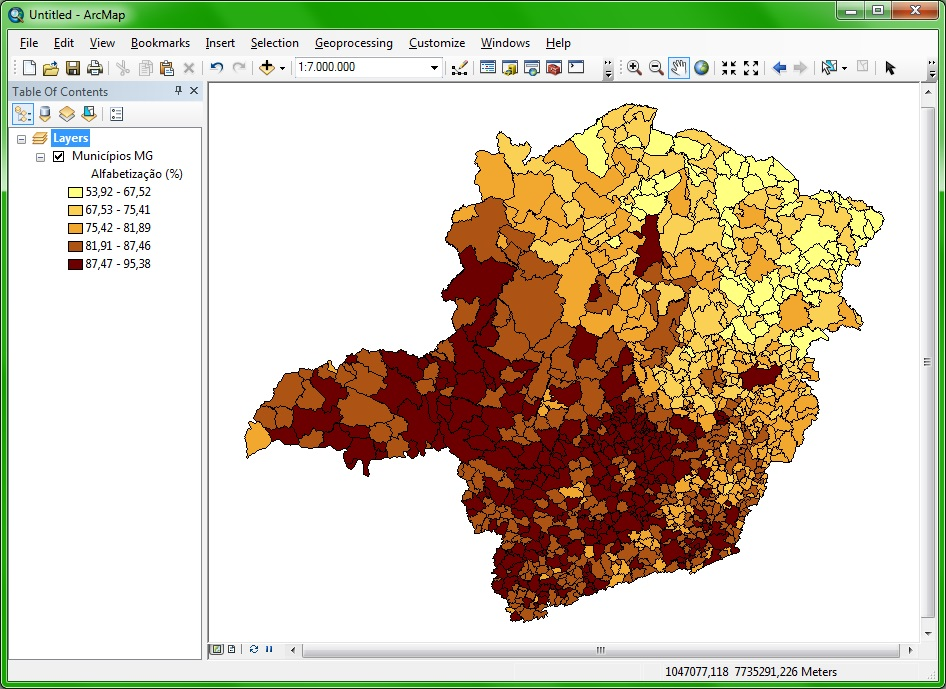
\includegraphics[scale=0.5]{ExemploArcGis.jpg}
\caption{ArcGIS utilizando mapa coroplético. Fonte: \citet{andersonm}.}
\label{arcgis}
\end{figure}

\subsection{API}

API (\emph{Application Program Interface})\footnote{em português, Interface de Programação de Aplicativos.} é um conjunto de rotinas, protocolos (padrões de programação) e ferramentas para criar aplicativos e softwares. Uma API especifica como os componentes de software devem interagir. Uma boa API torna mais fácil desenvolver um programa fornecendo todos os métodos de construção \citep{canaltechapi}.

Existem muitos tipos diferentes de APIs para sistemas operacionais, aplicativos ou sites. O Windows, por exemplo, tem muitos conjuntos de API que são usados pelo hardware e aplicativos do sistema. Na \emph{Web} ela funciona como um serviço na qual uma aplicação faz uma requisição aos métodos e a API retorna um valor de resposta.

Um estudo feito ainda pelo \citeauthor{canaltechapi} diz que, recentemente, a utilização das APIs tem se espalhado nos plug-ins, que complementam a funcionalidade de um determinado programa. Os desenvolvedores de um programa principal criam uma API específica e fornecem a outros criadores, que desenvolvem plug-ins para aumentar o potencial e as funcionalidades do programa.

\subsection{Padrões e Tecnologias \emph{Web}}

Padrões \emph{Web} ou \emph{Standard Web} são um conjunto de normas e recomendações de boas práticas de desenvolvimento, com o objetivo de padronizar e criar uma \emph{Web} ``universal". Ela define basicamente o que usar, quando usar e como usar. O \citet{w3c} é o órgão que regulamenta esses padrões.

Dentre as tecnologias padronizadas, existem algumas que se destacam pelo crescente uso global e são a base de todas as outras. São elas:

\begin{itemize}
\item HTML: \emph{HyperText Markup Language} é a linguagem usada para descrever e definir o conteúdo de uma página da \emph{Web} em um formato bem estruturado;
\item CSS: \emph{Cascading Style Sheets} são usados para descrever a aparência do conteúdo da \emph{Web};
\item JavaScript: é a linguagem de programação que é executada no navegador, usado para construir sites interativos avançados e aplicativos para a execução segura do navegador.
\end{itemize}

\section{Trabalhos Relacionados}

Nesta seção serão apresentados alguns trabalhos relacionados ao tema proposto.

\citet{cancado} apresentou uma tese que propunha um método que permitisse a realização de análises espaciais das interrupções no abastecimento de água do município de Belo Horizonte. Foram utilizados para a resolução do problema conceitos relacionados ao SIG, em especial as relações de proximidade e continência.

\citet{laudares} teve como objetivo em seu trabalho a investigação e classificação de componentes genéricos para Geovisualização na \emph{Web} e a organização de um ambiente virtual utilizado como repositório para dar suporte à geração de SIGs na Internet, comprovando a aplicabilidade e eficácia do uso desses componentes através da utilização em estudos de caso. \citeauthor{laudares} conclui que existe um aumento na utilização de componentes genéricos padronizados para o desenvolvimento de sistemas de Geovisualização, e afirma que o uso desses componentes no desenvolvimento de soluções para análise e visualização de dados espaciais visa atender os requisitos de padronização, uma vez que eles permitem que sistemas executados em diferentes ambientes que se comuniquem pelo mesmo padrão \emph{Web}.

\citet{santos} realizou em sua dissertação uma pesquisa que buscasse responder o seguinte problema: de que maneira a representação digital da informação geográfica na \emph{Web} colabora para a construção do conhecimento cientifico? Trata-se de uma pesquisa de nível exploratório e descritivo, onde ele utilizou de registros bibliométricos como fontes de dados e métodos cientométricos para a coleta e a análise dos dados. Utilizou também o \emph{software VOSViewer} para visualização do mapa de termos, fazendo uso da metáfora de distância utilizados em mapas tradicionais para representar os relacionamentos entre os termos. \citeauthor{santos} conclui que houve uma tendência de crescimento da quantidade de trabalhos acadêmicos relacionados à RDIG, o que sustenta a hipótese de colaboração da representação digital da informação geográfica à construção do conhecimento científico.

\citet{kutova} desenvolveu uma biblioteca (GeoPUCMinas) com recursos em JavaScript para a produção de mapas e para análises espaciais, que pode ser incorporado a qualquer página \emph{Web}. Com o objetivo de análise espacial dos cursos superiores e das matrículas nesses cursos nos municípios do estado de Minas Gerais, \citeauthor{kutova} também desenvolveu o Mapeamento da Educação Superior (MAPES), que integrado a essa biblioteca, era possível obter várias formas de representação de dados, como mapas e gráficos, do Censo Demográfico 2010 do IBGE\footnote{Instituto Brasileiro de Geografia e Estatística.} e do Censo de Educação Superior 2010 do INEP\footnote{Instituto Nacional de Estudos e Pesquisas Educacionais Anísio Teixeira.}.

Dados os trabalhos acima citados, o diferencial deste projeto se dá pela pretenção de criar uma plataforma \emph{Web} utilizável por qualquer tipo de usuário, independente de seu conhecimento em SIGs. Nela será possível visualizar dados de qualquer área do território brasileiro, desde regiões à municípios, apenas selecionando a região escolhida e inserindo uma base de dados referente (de acordo com os formatos de arquivos permitidos, explicitados na seção \ref{metodologia}), obtendo assim estruturas contendo informações concretas para análise dos mesmos.

\section{Metodologia} \label{metodologia}

Este trabalho apresentará o desenvolvimento de uma API e uma pesquisa experimental descritiva, onde dados serão inseridos, analisados e interpretados, por meio do material a ser desenvolvido.

\subsection{Etapas da Pesquisa} \label{atividades}

Esta pesquisa será divida nas seguintes etapas / atividades:

\begin{enumerate}[I]
  \item{Levantamento de requisitos;}  
  \item{Modelagem do sistema;}
  \item{Desenvolvimento do sistema;}  
  	\begin{enumerate}
    	\item{Criação e leitura da base de mapas brasileiros;}  
        \item{Métodos para desenho poligonal;}  
        \item{Carregamento dos dados e aplicação em mapas dinâmicos e interativos;} 
    	\item{Desenvolvimento da aplicação \emph{Web} de teste;} 
  	\end{enumerate}
  \item{Teste do sistema;}  
  \item{Teste de usabilidade do sistema;}  
  \item{Apresentação e análise dos resultados.}
\end{enumerate}

No levantamento de requisitos será feita uma análise junto a dois professores especialistas no assunto para levantar quais as características e funcionalidades necessárias à API, informações sobre o tipo de dados e sua origem, além de outras informações voltadas ao sistema (requisitos não funcionais).

Na etapa de modelagem do sistema serão elaborados Diagramas de Casos de Uso e de Entidade e Relacionamento (DER), com propósito de facilitar o processo de desenvolvimento da aplicação.

O desenvolvimento do sistema será efetivamente a construção da API e da aplicação teste. Serão avaliadas as tecnologias disponíveis e selecionadas aquelas que melhor se adequarem aos requisitos. A subseção \ref{tecnologias} explicitará melhor essa escolha.

O teste do sistema consiste em carregar diferentes arquivos de dados para verificar suas compatibilidades com os diferentes tipos de mapas da base e fazer prova e validação de cada uma das funções e métodos desenvolvidos.

Na etapa de teste de usabilidade do sistema, o mesmo será submetido à algumas pessoas para qual este sistema seria interessante. Eles deverão utilizar as funcionalidades do sistema e logo após, lhes serão aplicados um questionário referente a usabilidade do mesmo.

Ao término, os resultados dos testes serão apresentados em gráficos e, por fim, analisados.

\subsection{Ambiente de Desenvolvimento} \label{tecnologias}

Para desenvolver a API com as características necessárias para este trabalho, é preciso avaliar as tecnologias atuais para encontrar as que mais se adequam ao projeto. Essa avaliação foi realizada em três etapas, conforme descrito a seguir.

A primeira etapa é a definição de uma plataforma de visualização de dados. Essa plataforma deve permitir visualizar dados tanto de macrorregiões, como países e estados, quanto de meso e microrregiões, como áreas metropolitanas e municípios, sendo que estes dados devem ser impressos sobre um mapa coroplético e formas de gráficos. Desta maneira, será utilizada a biblioteca D3.js, e sua extensão D3.geo. Com as duas é possível criar mapas temáticos e interativos com apoio de gráficos.

A segunda etapa é quanto ao tipo de arquivo de mapas. É preciso observar a compatibilidade do arquivo com a plataforma de visualização e como são representados os objetos gráficos no tipo de arquivo (pontos, linhas, polígonos, altitude, longitude, etc.). O formato que mais atende aos requisitos é o TopoJson, uma simplificação GeoJson, tanto em informações quanto no tamanho do arquivo. A API ainda suportará arquivos nos formatos GeoJson e Shapefile, pois os mesmos poderão ser convertidos pela API para o formato TopoJson. Para fazer a leitura dos arquivos e realizar as conversões, será utilizado o npm, um gerenciador de pacotes da biblioteca Node.js. Ele é capaz de buscar e importar pacotes necessários na aplicação, fazendo as atualizações quando necessárias.

Por fim, a terceira etapa é quanto ao desenvolvimento da aplicação teste. Uma simples aplicação \emph{Web} será desenvolvida para testar e validar a API. Essa aplicação será feita com padrões HTML, CSS e JavaScript. Para melhorar a interação com o usuário, será utilizado o framework JavaScript JQuery, pois possui recursos que permitirão criar animações e produzir efeitos na tela de acordo com as ações do usuário.

Além disso, para inserir o arquivo a ser visualizado, será utilizado o formato CSV, onde os dados serão convertidos em JSON, e feito as aplicações aos mapas.

A Tabela \ref{tabtecnologias} apresenta um resumo das tecnologias e recursos que serão utilizados.

\begin{table}[!htbp]
	\centering
    \caption{Ferramentas do ambiente de desenvolvimento}
	\begin{tabular}{|c|c|}
    \hline
    \multicolumn{1}{|c|}{{\cellcolor[rgb]{.75, .75, .75} \textbf{Funcionalidades}}} & \multicolumn{1}{|c|}{{\cellcolor[rgb]{.75, .75, .75} \textbf{Ferramentas}}}
    \tabularnewline \hline
      Plataforma de visualização de dados & D3.js \tabularnewline \hline
      Formato de arquivos de mapas & TopoJson, GeoJson e Shapefile \tabularnewline \hline
      Formato de arquivos de dados & CSV e JSON \tabularnewline \hline
      Programação \emph{Web} & HTML, CSS e JavaScript \tabularnewline \hline
      Gerenciador de pacotes & Node.js (npm) \tabularnewline \hline
	\end{tabular}
    \label{tabtecnologias}
\end{table} 

\subsection{Cronograma}

Para realização das atividades já referenciadas na subseção \ref{atividades}, foi proposto um cronograma de acordo com o tempo previsto de execução de cada uma, apresentado na Tabela \ref{tabcronograma}.

%\begin{table}[htbp]
%	\centering
%    \caption{Cronograma de atividades}
%	\begin{tabular}{|c|c|c|c|c|c|c|}
%      \hline
%      \multicolumn{1}{|c|}{\multirow{2}[4]{*}{\textbf{Atividades}}} & \multicolumn{6}{c|}{\textbf{Período}} \tabularnewline 
%      \cline{2-7} & \textbf{Jun/17} & \textbf{Jul/17} & \textbf{Ago/17} & \textbf{Set/17} & \textbf{Out/17} & \textbf{Nov/17} \tabularnewline \hline
%      I 	& \cellcolor[rgb]{.75, .75, .75}x x x &  &  &  &  & \tabularnewline \hline
%      II 	& \cellcolor[rgb]{.75, .75, .75}x x x &  &  &  &  & \tabularnewline \hline
%      III-a &  & \cellcolor[rgb]{.75, .75, .75}x x x &  &  &  & \tabularnewline \hline
%      III-b &  & \cellcolor[rgb]{.75, .75, .75}x x x & \cellcolor[rgb]{.75, .75, .75}x x x &  &  & \tabularnewline \hline
%      III-c &  &  & \cellcolor[rgb]{.75, .75, .75}x x x & \cellcolor[rgb]{.75, .75, .75}x x x &  & \tabularnewline \hline
%      III-d &  &  &  & \cellcolor[rgb]{.75, .75, .75}x x x &  & \tabularnewline \hline
%      IV 	&  &  &  &  & \cellcolor[rgb]{.75, .75, .75}x x x & \tabularnewline \hline
%      V 	&  &  &  &  & \cellcolor[rgb]{.75, .75, .75}x x x &  \tabularnewline \hline
%      VI 	&  &  &  &  &  & \cellcolor[rgb]{.75, .75, .75}x x x \tabularnewline \hline
%	\end{tabular}
%    \label{tabcronograma}
%\end{table}

\begin{table}[!htbp]
	\scalefont{0.8}
	\centering
    \caption{Cronograma de atividades}
	\begin{tabular}{|>{\centering\arraybackslash}m{0.7cm}|>{\arraybackslash}m{5cm}|>{\centering\arraybackslash}m{0.9cm}|>{\centering\arraybackslash}m{0.9cm}|>{\centering\arraybackslash}m{0.9cm}|>{\centering\arraybackslash}m{0.9cm}|>{\centering\arraybackslash}m{0.9cm}|>{\centering\arraybackslash}m{0.9cm}|}
     \hline
     \multicolumn{1}{|c|}{\multirow{2}{*}{\textbf{Item}}} & \multicolumn{1}{c|}{\multirow{2}{*}{\textbf{Atividades}}} & \multicolumn{6}{c|}{\textbf{Período}} \\
     \cline{3-8} & & \textbf{Jun/17} & \textbf{Jul/17} & \textbf{Ago/17} & \textbf{Set/17} & \textbf{Out/17} & \textbf{Nov/17} \\ \hline
      I & Levantamento de requisitos & \cellcolor[rgb]{.75, .75, .75}x x x &  &  &  &  & \\ \hline
      II & Modelagem do sistema & \cellcolor[rgb]{.75, .75, .75}x x x &  &  &  &  & \\ \hline
      III-a & Criação e leitura da base de mapas brasileiros &  & \cellcolor[rgb]{.75, .75, .75}x x x &  &  &  & \\ \hline
      III-b & Métodos para desenho poligonal &  & \cellcolor[rgb]{.75, .75, .75}x x x & \cellcolor[rgb]{.75, .75, .75}x x x &  &  & \\ \hline
      III-c & Carregamento dos dados e aplicação em mapas dinâmicos e interativos &  &  & \cellcolor[rgb]{.75, .75, .75}x x x & \cellcolor[rgb]{.75, .75, .75}x x x &  & \\ \hline
      III-d & Desenvolvimento da aplicação \emph{Web} de teste &  &  &  & \cellcolor[rgb]{.75, .75, .75}x x x &  & \\ \hline
      IV & Teste do sistema &  &  &  &  & \cellcolor[rgb]{.75, .75, .75}x x x & \\ \hline
      V & Teste de usabilidade do sistema &  &  &  &  & \cellcolor[rgb]{.75, .75, .75}x x x & \\ \hline
      VI & Apresentação e análise dos resultados &  &  &  &  &  & \cellcolor[rgb]{.75, .75, .75}x x x \\ \hline
	\end{tabular}
    \label{tabcronograma}
\end{table}

% \cellcolor[rgb]{1, .753, 0} 

Pretende-se ao término do segundo semestre de 2017 realizar a apresentação do projeto em pleno funcionamento, testado e validado. Posteriormente, será possível disponibilizar a plataforma para o uso acadêmico em pesquisas e rotinas de estudos.

\pagebreak

\bibliographystyle{apa}
\bibliography{referencias}

\end{document}